\documentclass[tikz,border=8pt]{standalone}
\usepackage{xcolor}
\usetikzlibrary{calc,arrows.meta,backgrounds}
\definecolor{bg}{HTML}{1B1F27}
\definecolor{fg}{HTML}{E6EDF3}
\definecolor{dim}{HTML}{9AA5B1}
\definecolor{c1}{HTML}{7BC47F}
\definecolor{c2}{HTML}{E5826F}
\definecolor{cd}{HTML}{B39DDB}
\definecolor{feat}{HTML}{F0C060}
\begin{document}
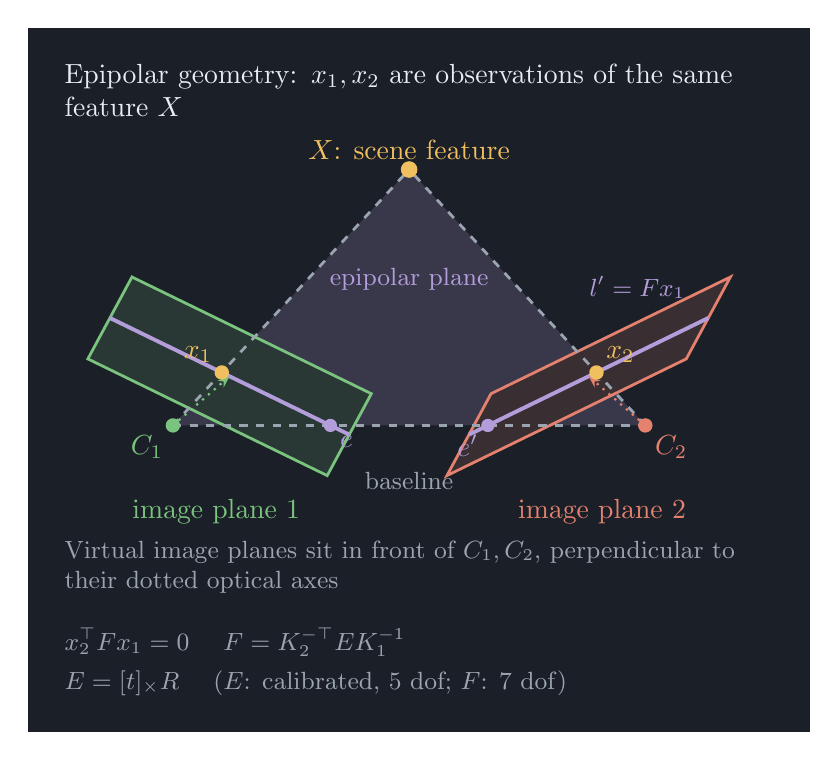
\begin{tikzpicture}[x={(1cm,0cm)}, y={(0.35cm,0.65cm)}, z={(0cm,0.65cm)}, show background rectangle, background rectangle/.style={fill=bg}, inner frame sep=10pt, every node/.style={text=fg}]
\def\focal{1.2}
\def\halfwidth{1.9}
\def\halfheight{0.8}
\coordinate (C1) at (-3,0,0);
\coordinate (C2) at (3,0,0);
\coordinate (X) at (0,0,5);
\fill[cd!20!bg] (C1) -- (C2) -- (X) -- cycle;

% Unit normals n_k=(+/-0.6,0,0.8); image axes u_k=(0.8,0,-/+0.6), v=(0,1,0).
\foreach \k/\cx/\s in {1/-3/1,2/3/-1}{
  \coordinate (O\k) at (\cx+\s*0.6*\focal,0,0.8*\focal);
  \foreach \corner/\u/\v in {a/-1/-1,b/1/-1,c/1/1,d/-1/1}{
    \coordinate (P\k\corner) at (\cx+\s*0.6*\focal+0.8*\u*\halfwidth,\v*\halfheight,0.8*\focal-\s*0.6*\u*\halfwidth);
  }
  \coordinate (L\k-a) at (\cx+\s*0.6*\focal-0.8*\halfwidth,0,0.8*\focal+\s*0.6*\halfwidth);
  \coordinate (L\k-b) at (\cx+\s*0.6*\focal+0.8*\halfwidth,0,0.8*\focal-\s*0.6*\halfwidth);
}
\draw[c1, line width=1pt, fill=c1!15!bg] (P1a) -- (P1b) -- (P1c) -- (P1d) -- cycle;
\draw[c2, line width=1pt, fill=c2!15!bg] (P2a) -- (P2b) -- (P2c) -- (P2d) -- cycle;

% q=f/(n_k dot (X-C_k)); the baseline intersections use n_k dot (C_other-C_k).
\pgfmathsetmacro{\featurefraction}{\focal/(0.6*3+0.8*5)}
\pgfmathsetmacro{\baselinefraction}{\focal/(0.6*6)}
\coordinate (x1) at ($(C1)!\featurefraction!(X)$);
\coordinate (x2) at ($(C2)!\featurefraction!(X)$);
\coordinate (e1) at ($(C1)!\baselinefraction!(C2)$);
\coordinate (e2) at ($(C2)!\baselinefraction!(C1)$);

\draw[dim, dashed, line width=0.9pt] (C1) -- (C2);
\draw[dim, dashed, line width=1pt] (C1) -- (X);
\draw[dim, dashed, line width=1pt] (C2) -- (X);
\draw[cd, line width=1.4pt] (L1-a) -- (L1-b);
\draw[cd, line width=1.4pt] (L2-a) -- (L2-b);
\draw[c1, dotted, -{Stealth[length=1.5mm]}, line width=0.8pt] (C1) -- (O1);
\draw[c2, dotted, -{Stealth[length=1.5mm]}, line width=0.8pt] (C2) -- (O2);

\fill[c1] (C1) circle (2.6pt);
\fill[c2] (C2) circle (2.6pt);
\node[text=c1, below left] at (C1) {$C_1$};
\node[text=c2, below right] at (C2) {$C_2$};
\fill[feat] (X) circle (3pt);
\node[text=feat, above] at (X) {$X$: scene feature};
\fill[feat] (x1) circle (2.6pt);
\fill[feat] (x2) circle (2.6pt);
\node[text=feat, above left] at (x1) {$x_1$};
\node[text=feat, above right] at (x2) {$x_2$};
\fill[cd] (e1) circle (2.4pt);
\fill[cd] (e2) circle (2.4pt);
\node[text=cd, below right] at (e1) {$e$};
\node[text=cd, below left] at (e2) {$e'$};
\node[text=cd, font=\small] at (canvas cs:x=0cm,y=1.85cm) {epipolar plane};
\node[text=dim, font=\small] at (canvas cs:x=0cm,y=-0.7cm) {baseline};
\node[text=c1] at (canvas cs:x=-2.45cm,y=-1.1cm) {image plane 1};
\node[text=c2] at (canvas cs:x=2.45cm,y=-1.1cm) {image plane 2};
\node[text=cd, font=\small] at (canvas cs:x=2.9cm,y=1.75cm) {$l'=Fx_1$};
\node[anchor=west, align=left, text width=9cm] at (canvas cs:x=-4.5cm,y=4.25cm) {Epipolar geometry: $x_1,x_2$ are observations of the same feature $X$};
\node[anchor=west, align=left, text width=9cm, text=dim, font=\small] at (canvas cs:x=-4.5cm,y=-1.8cm) {Virtual image planes sit in front of $C_1,C_2$, perpendicular to their dotted optical axes};
\node[anchor=west, align=left, text=dim, font=\small] at (canvas cs:x=-4.5cm,y=-3.0cm) {$x_2^{\top}Fx_1=0$ \quad $F=K_2^{-\top}EK_1^{-1}$\\[3pt] $E=[t]_\times R$ \quad ($E$: calibrated, 5 dof; $F$: 7 dof)};
\end{tikzpicture}
\end{document}
